\documentclass{article}
\usepackage{amsmath}
\usepackage{graphicx}
\usepackage[table]{xcolor}
\begin{document}
	\begin{titlepage}
			\title{\huge{Logic Gates}}
		\author{Dumebi Valerie Duru}
		\maketitle
		\begin{figure}[t!]
			\centering
			
\includegraphics[width=0.9\linewidth]{pictures/pau logo.png}
		\end{figure}
	\end{titlepage}
	
	
		
		\tableofcontents
		
		\newpage
		\section{Logic Gates}
			A logic gate is a building block of a digital circuit which is at the heart of any computer operation. Behind every digital system is a logic gate.Logic gates perform logical operations that take binary input (0s and 1s) and produce  a single binary output. They are used in most electronic device including:
				\begin{table}[h!]
					\begin{center}
						\label{tab: table 1}
						\begin{tabular}{c c c}
							\hline
							\textcolor{red}{Smartphones} & \textcolor{green}{Tablets} & \textcolor{blue}{Memory Devices}\\
							\hline
							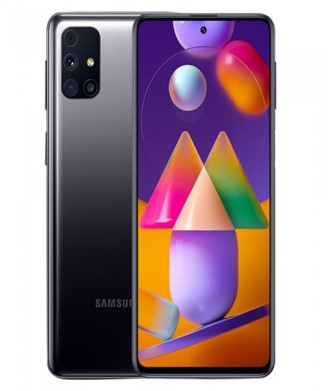
\includegraphics[width=0.1\linewidth]{pictures/phone.jpg} & 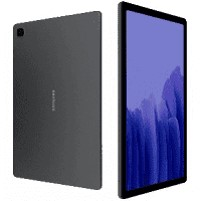
\includegraphics[width=0.1\linewidth]{pictures/tablet.jpg} & 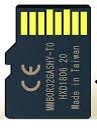
\includegraphics[width=0.1\linewidth]{pictures/memory device.jpg}\\
							\hline
						\end{tabular}
					\end{center}	
				\end{table}
		\newline
			Now think of a logic gate like a light switch, it is either in an ON or OFF position. Similarly, the input output terminals are always in one of two binary positions false(0) and true(1). Each gate has its own logic or set of rules that determines how it acts based on multiple inputs outlined in a truth table.
		\newpage	
		\section{Types of Logic Gates}
			Fundamental gates are \textbf{AND, OR and NOT}
			Derived Gates are \textbf{NAND, NOR, XOR and XNOR} (derived from the fundamental gates)
			
			Universal Gates are\textbf{NAND and NOR gates} (the fundamental logic gates can be realized through them).
			
			\subsection{Fundamental Gates}
				\subsubsection{AND Gate}
					The expression C = A X B reads as “C equals A AND B“ 
					The multiplication sign (X) stands for the AND operation, same for ordinary multiplication of 1s and 0s.\newline
						\begin{figure}[h!]
							\begin{center}
								\caption{AND Gate}
								\label{fig 1: AND gate}
								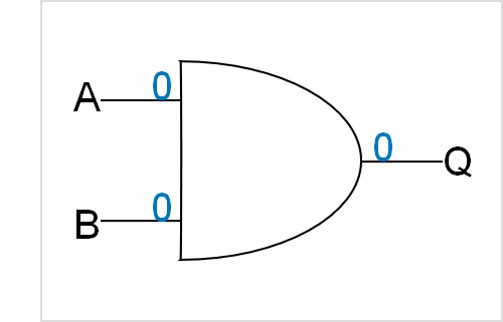
\includegraphics[width=0.5\linewidth]{pictures/AND Gate.jpg}
							\end{center}
						\end{figure}
					
					The AND operation produces a true output (result of 1) only for the single case when all of the input variables are 1 and a false output (result of 0) where one or more inputs are 0.
					
				\subsubsection{OR Gate}
					The expression C = A + B reads as “C equals A OR B". It is the inclusive “OR”
					The Addition (+) sign stands for the OR operation. \newline
						\begin{figure}[h!]
							\caption{OR Gate}
							\label{fig 2: OR Gate}
							\begin{center}
								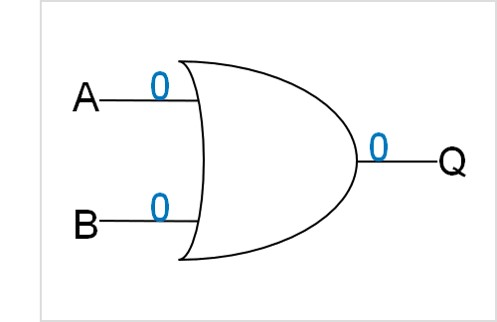
\includegraphics[width=0.5\linewidth]{pictures/OR Gate.jpg}
							\end{center}
						\end{figure}
						
					The OR operation produces a true output (result of 1) when any of the input variable is 1 and a false output (result of 0) only when all the input variables are 0.
				\newpage	
				\subsubsection{NOT Gate}
					The NOT gate is called a logical inverter.
					It has only one input. It reverses the original input (A) to give an inverted output C.
					\begin{figure}[h!]
						\begin{center}
							\caption{NOT Gate}
							\label{fig 3: NOT Gate}
							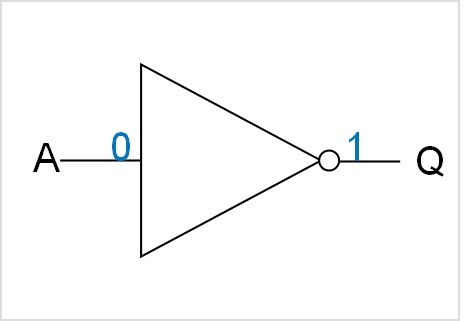
\includegraphics[width=0.5\linewidth]{pictures/NOT gate.jpg}
						\end{center}
					\end{figure}
				
			\subsection{Derived Gates}
				\subsubsection{NOR Gate}
					The NOR (NOT OR) gate circuit is an inverter OR gate
					\begin{center}
						\begin{math}
							C = \overline{A+B}
						\end{math}
					\end{center}
				
					Reads as C = NOT of A or B
					
					The NOR Gate gives a true output (result of 1) only when both inputs are false (0)
					
					\textcolor{red}{The NOR Gate is a universal gate because it can be used to form any other kind of gate}
					\begin{figure}[h!]
						\caption{NOR Gate}
						\label{fig 4: NOR Gate}
						\begin{center}
							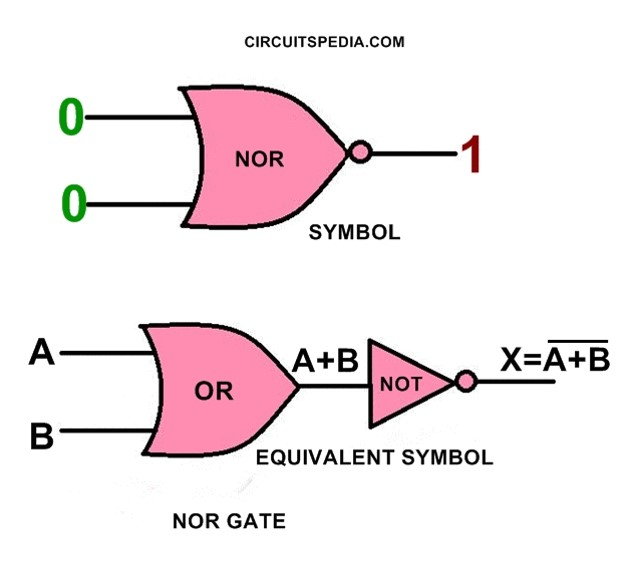
\includegraphics[width=0.5\linewidth]{pictures/NOR Gate.jpg}
						\end{center}
					\end{figure}
					
				\subsubsection{NAND Gate}
					The NAND (NOT AND) Gate is an inverted AND Gate
					\begin{center}
						\begin{math}
							C = \overline{A * B}
						\end{math}
					\end{center}
					Reads as C = NOT of A AND B
					The NAND Gate gives a false output (result of 0) only when both inputs are true (1)
					\newline
					\textcolor{red}{The NAND Gate is a universal gate because it can be used to form any other kind of gate.}
						\begin{figure}[h!]
							\caption{NAND Gate}
							\label{fig 5: NAND Gate}
							\begin{center}
								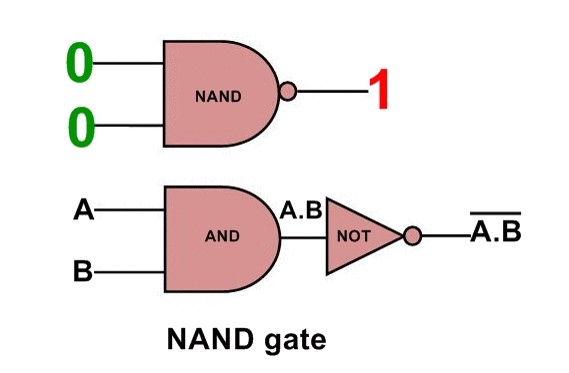
\includegraphics[width=0.5\linewidth]{pictures/NAND Gate.jpg}
							\end{center}
						\end{figure}
				
				\subsubsection{XOR Gate}
					An XOR (exclusive OR) gate acts in the same way as the exclusive OR logical connector. 
					It gives a true output (result of 1) if one, and only one, of the inputs to the gate is true (1), i.e either or but not both
						\begin{center}
							\begin{math}
								C = \overline{A}.B + \overline{B}.A
							\end{math}
						\end{center}
					
						\begin{table}[h!]
							\centering
							\caption{XOR Truth Table}
							\label{tab 2: XOR table}
							\begin{tabular}{|c|c|c|c|c|c|c|}
								
							\rowcolor{blue!60}	A & B & $\overline{A}$ & $\overline{A}$.B & $\overline{B}$ & $\overline{B}$.A & C = $\overline{A}$.B + $\overline{B}$.A  \\
								\hline
							\rowcolor{blue!10}	0 & 0 & 1 & 0 & 1 & 0 & 0\\
							\rowcolor{blue!20}	1 & 0 & 0 & 0 & 1 & 1 & 1\\
							\rowcolor{blue!10}	0 & 1 & 1 & 1 & 0 & 0 & 1\\
							\rowcolor{blue!20}	1 & 1 & 0 & 0 & 0 & 0 & 0 \\ \hline
								
							\end{tabular}
						\end{table}
					
				\subsubsection{XNOR Gate}
					The XNOR (exclusive - NOR) gate is a combination XOR gate followed by an inverter. 
						\begin{center}
							\begin{math}
								C= \overline{\overline{A}.B + \overline{B}.A}
							\end{math}
						\end{center}
					
						\begin{table}[h!]
							\centering
							\caption{XNOR Truth Table}
							\label{tab 3: XNOR table}
							\begin{tabular}{|c|c|c|c|c|c|c|c|}
								
							\rowcolor{blue!60}	A & B & $\overline{A}$ & $\overline{A}$.B & $\overline{B}$ & $\overline{B}$.A & $\overline{A}$.B + $\overline{B}$.A & C = $\overline{\overline{A}.B + \overline{B}.A}$  \\
								\hline
							\rowcolor{blue!10}	0 & 0 & 1 & 0 & 1 & 0 & 0 & 1\\
							\rowcolor{blue!20}	1 & 0 & 0 & 0 & 1 & 1 & 1 & 0\\
							\rowcolor{blue!10}	0 & 1 & 1 & 1 & 0 & 0 & 1 & 0\\
							\rowcolor{blue!20}	1 & 1 & 0 & 0 & 0 & 0 & 0 & 1 \\ \hline
								
							\end{tabular}
						\end{table}
		\newpage
		\section{Logic Gates and Their Truth Tables}
			\begin{figure}[h!]
				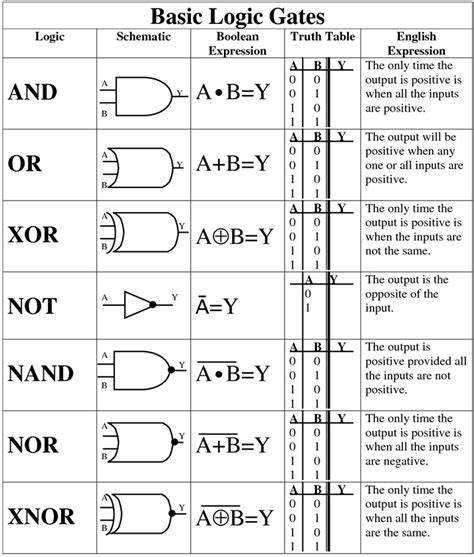
\includegraphics[width=1\linewidth]{pictures/Logic gate and truth table.jpg }
				\cite{picture}
			\end{figure}
		\newpage

		\section{Summary}
			\begin{itemize}
				\item{Using different combination of logic gates, complex operations can be performed.}
				\item{With the Universal logic gates - NAND and NOR, any other gate can be built}
				\item{There is no limit to the number of gates that can be arranged together in a single device.}	
				\item{However, in practice, there is a limit to the number of gates that can be packed into a given physical space.}	 
				\item{Arrays of logic gates are found in digital integrated circuits.}	
				\item{The logic gates are abstract representations of real electronic circuits}
				\item{In computers, Logic gates are built using transistors combined with other electrical components like resistors and diodes.}
				\item{These electrical components are wired together in order to transform a particular input to give a desired output}
				
			\end{itemize}
		\newpage
		\section{Quiz}
			\begin{enumerate}
				\item{What is the output of an AND gate if the inputs are 1 and 0?}
				\item{Explain the difference between the AND gate and the OR gate.}
				\item{What is the output of a NOT gate if the inputs is 0?}
				\item{Which logic gate is this?}
				\item{Which gate is also known a logical converter?}
			\end{enumerate}
		\cite{logicgates2021}
		\cite{logicgates}
		\newpage
		\bibliography{logicGates.bib}	
		\bibliographystyle{ieeetr}
		
		
		
\end{document}